\documentclass[a4paper, 12pt]{article}
\usepackage[utf8]{inputenc}
\usepackage[T2A]{fontenc}
\usepackage{amsmath,amssymb,amsthm}
\usepackage[a4paper,hmargin=2.5cm,vmargin=2.5cm]{geometry}
\usepackage[english]{babel}
% \usepackage{graphics}
\usepackage{float}
\usepackage{graphicx}


\DeclareMathOperator{\argmax}{argmax}
\DeclareMathOperator{\Image}{Im}


\graphicspath{{./images/}}

\theoremstyle{definition}
\newtheorem{definition}{Definition}[section]


\theoremstyle{definition}
\newtheorem{example}{Example}[section]

\newtheorem{theorem}{Theorem}

\theoremstyle{remark}
\newtheorem*{remark}{Remark}

\usepackage{xcolor}
\newcommand\myworries[1]{\textcolor{red}{#1}}

\begin{document}

%%
%% Title page
%%
\begin{center}
{\scshape National Research University\\
Higher School of Economics\\[1ex]
Faculty of Mathematics\par}

\par\vfill

\textbf{\large Project Proposal}

\vspace{1.5cm}

{\Large\bfseries
Clustering of Multidimensional Random Variables to Improve HMM Sequence Alignment Accuracy \\

Кластеризация многомерной случайно величины для поднятия точности выравнивания строк.
\par}

\vspace{1.5cm}

\par\vfill
\noindent\hspace{0.52\textwidth}\parbox[t]{0.48\textwidth}{%
Student: Denis Grachev, БМТ181\\[2ex]
}

\par\vfill
\noindent\hspace{0.52\textwidth}\parbox[t]{0.48\textwidth}{%
Scientific advisor:\\[3pt]
PhD candidate, \\ 
Timofey Prodanov\\[2ex]
}

\par\vfill\vfill
Moscow 2022
\end{center}
\thispagestyle{empty}
\pagebreak

%%
%% ===========================================================================
%%

\tableofcontents
\newpage

\section{Abstract}

Whole-genome sequencing is an complex and important task of bioinformatics. 
Different technologies can generate data of different nature. 
Most popular technologies, such as illumina, 
have low error rate, but give limited information about genome.
Newer techologies, for example Pacific Biosciences and Oxford Nanopore, 
can give more details about genome, but have higher error rate. 
Combination of these methods can help improve accuracy of genome sequencing. 
During this work a new method of string clustering was developed, 
to identify different data profiles and new functionality to existing tools were added,
to work with multiple datasets. 


\section{Introduction}
Bioinformatics is an interdisciplinary science that aims 
to develops methods and software tools 
for understanding biological data. 
One of the ways to model haploid genome is to present it as 
pair of sequences or strings over the alphabet $\{ A, C, G, T \}$. 
Modern technologies of reading genome do not sequence it as one 
continious string, but a number of random overlaping substrings 
that are called reads. 
As within one biological species genomes coincide almost completely, 
it is convenient to determine one reference genome for one species 
and identify for every individual it's deviations from the reference.
These single nucleotide variants are called SNVs.  
Taking into cosideration these facts and the fact that various 
errors happen during all stages of the process, a number of 
problems appears for example:
\begin{itemize}
    \item \textbf{Genome assembly} is process of  
    deciphering genome using reads obtained from it.
    
    \item \textbf{Sequence alignment} is process of 
    arranging sequences to spot similarities between them. 
    
    \item \textbf{Variant calling} is process of identifying 
    SNVs of an individual based on reads aligned on the reference genome.
\end{itemize}

The most commonly used technologies nowadays, 
such as illumina, allow to sequence reads of length 200-500 bp.
Sequencing human genome using such short length reads 
has many limitations. 
First, due to diploidy of humans, it is important to obtain
long-range haplotype information. This might be difficult 
with short-reads provided by illumina. Secondly $~3.6\%$ of 
human genome consists of long highly repetative 
duplicated regeions that can not be uniquely aligned, 
which lowers accuracy of SNVs. 
Third-generation single-molecule sequencing (SMS) techologies,
such as Oxford Nanopore Technologies allow to   
genereate longer reads of length 10-30 kb. 
This techology might help overcome limitations that 
short-reads have. Variant calling tools that were developed 
for short-reads do not show high accuracy when applied 
to long-reads sequenced, due to significant difference 
in error rates and type of errors between these two types of reads. 
Also these tools process data in short windows 
of a few hundred bases lengths and not designed to agregate  
haplotype information present in long-reads, 
which might be crucial for distinguishing true deviations 
from errors.  

A number of new methods of variant calling were developed 
to work with long-reads, such as Deep Variant
and Longshot that uses deep learning 
and pair-Hidden Markov model algorithms to effectivly work with 
such data.  
Accuracy of these methods can be improved by agrigating 
information from multiple sequence data sets together. 
An example of effectiveness of such method is 
Spades genome assembly tool, which uses short and long 
read data together.  

Longshot works effectivly with one type of reads. 
To improve it's sencetivity and accuracy various 
methods of collecting data from diiferent sources 
can be applied. 
Previous research show that sequencing reads of 
different profiles and clustering them 
by their profiles can improve variant calling accuracy.

During this work we are going to extend functionality of 
Longshot tool to work effectivly with multiple datasets. 
For that we have to develop clustering algorithm for 
read profiles and implement such feature into Longshot. 

\section{Preliminaries}
\subsection{Strings}

\begin{definition}
    String is a sequence of letters of finite size. \\
    String of length $l$ over alphabet $A = \{ 1 \ldots m \}$ is a map $s: \{ 1 \ldots l\} \rightarrow A$.
    Usually elements of $A$ are denoted as characters for convenience.
\end{definition}

\begin{definition}
    Alignment of strings is a way of representing them to spot similarities. \\
    Alignment of strings $s_1$ and $s_2$ of lengths $l_1$ and $l_2$ respectively, 
    over alphabet $A$ is a pair of strings $\hat{s}_1$ and $\hat{s}_2$ 
    of length $l$ over alphabet $A \sqcup \{ '-' \}$, 
    such that there exists increasing functions $f_i: \{1 \ldots l_i \} \rightarrow \{ 1 \ldots l\}, i \in \{1, 2\}$ 
    such that $\hat{s}_i \circ f_i = s_i$ and $\Image (f_i) = \hat{s}_i^{-1}(A)$. \\
    
    Letter $'-'$ represents gap in a string. 
    String $\hat{s}_i$ represents string $s_i$ with inserted letter $'-'$, 
    that was not present in alphabet $A$, into some places, 
    and function $f_i$ maps indexes of letters in $s_i$ to corresponding indexes in $\hat{s}_i$.
\end{definition}

\begin{example}
    Alignment of strings $s_1 = CABCAABA$ and $s_2 = ABADBBAD$ 
    over alphabet $\{ A, B, C, D\}$.

    \begin{center}
        Initial strings. \\
        \begin{tabular}{|| c | c c c c c c c c ||}
         $s_1$ & C & A & B & C & A & A & B & A \\ 
         $s_2$ & A & B & A & D & B & B & A &   \\    
        \end{tabular}

        \hfill \break 

        Aligned strings. \\
        \begin{tabular}{|| c | c c c c c c c c c ||}
            $\hat{s}_1$ & C & A & B & C & - & A & A & B & A \\ 
            $\hat{s}_2$ & - & A & B & - & A & D & B & B & A   
        \end{tabular}

    \end{center}
\end{example}


% \begin{theorem}
%     If $G$ is symmetric and 
%     $
%     g_{ij} =
%         \left\{\begin{array}{cc}
%         0, & i = j\\
%         >0, & 
%         \end{array}\right.
%     $ and $p > 0$, then we can define metric for strings over alphabet $A$ as 
%     $$ d(s_1, s_2) = \min \{S(\hat{s}_1, \hat{s}_2)\}$$ 
% \end{theorem}

% \begin{proof}
    
% \end{proof}

\begin{definition}
    Define score function for an alignment $S(\hat{s}_1, \hat{s}_2)$. 
    The \emph{better} alignment the more score it gets. 
    Different score functions will be introduced later.
\end{definition}

\begin{definition}
    We are interested in the alignment with the highest possible score. 
    So we define score between two strings as 
    $$ S(s_1, s_2) = \max_{\hat{s}_1, \hat{s}_2} S(\hat{s}_1, \hat{s}_2 )$$ 
\end{definition}

\begin{definition}
    Substring is continious piece of a given string.\\
    For a string $s$ of length $l$, sub-string $s_s$ 
    is a string of length $l_s$, such that there exists a function
    $f: \{ 1 \ldots l_s \} \rightarrow \{ 1 \ldots l\}$
    such that
    $$ f(i) = i + d $$
    $$s \circ f = s_s.$$
\end{definition}

\begin{definition}
    We want to find similarities between reference string and reads. 
    For this we define local alignment and score for a string and a substring. \\  
    For a string $s_1$ and $s_2$ of lengths $l_1, l_2$ correspondingly, define string-sub-string score as 
    $$ S_s (s_1, s_2) = \max \{ S(s_s, s_2) | s_s \text{ is a sub-string of } s_1 \}$$
    and corresponding alignment $\hat{s}_1, \hat{s}_2$.
\end{definition}

\begin{definition}
    For a string $s$ of length $l$ and set of strings $R = \{ s_1 \ldots s_n \}$ 
    of lengths $\{ l_1 \ldots l_n \}$ correspondingly, 
    multiple alignment is tuple $\hat{s}, \hat{s}_1 \ldots \hat{s}_n$, 
    of strings of length $l$ over alphabet $A \sqcup \{ '-' \}$, such that $\sum_{i = 1}^n S(\hat{s}, \hat{s}_i)$ is maximal.
\end{definition}

\begin{definition}
    Set of reads $R$ for string $s$ of length $l$ and rate $r$ is 
    $$ R = \{ s_s | \text{length of } s_s > l, S_s(s, s_s) < r \}$$
\end{definition}

\subsection{Task}
Given reference string $s_r$ and reads $R$ for an unknown target string $s_t$, 
we know that $S(s_r, s_t) < D$ and whant to find $s_t$. \\

Plan:
\begin{enumerate}
    \item Make multiple alignment of $R$ over $s_r$.
    \item Estimate most likely difference between $s_r$ and $s_t$.
\end{enumerate}

\begin{figure}[H]
    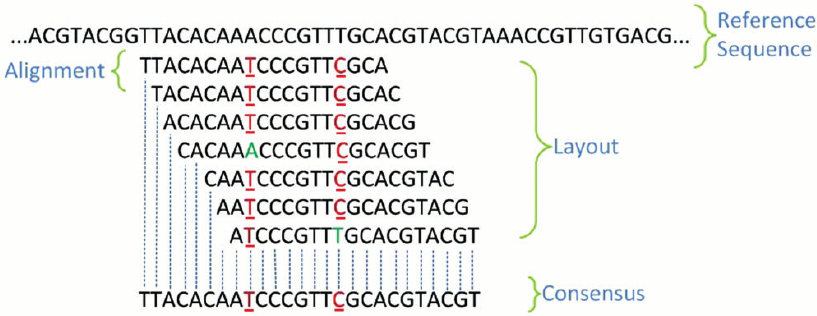
\includegraphics[scale=0.5]{aligned_reads.png}
    \centering
    \caption{Example of reference string, target string and reads.}
\end{figure}

\subsection{Additive scoring functions}

One of the ways to score an alignment is to add award for matches and 
subtract penalty for mismatches and gaps. 

\begin{definition}    
    For a given matrix $G \in \mathbb{R}^{|A \sqcup \{ '-' \} | \times |A \sqcup \{ '-' \}|}$ and $p \in \mathbb{R}$ 
    score of alignment $\hat{s}_1, \hat{s}_2$ is 
    $$ S(\hat{s}_1, \hat{s}_2) = \sum_{i = 1}^l G_{\hat{s}_1(i), \hat{s}_2(i)}. $$
    %     \text{ where } 
    %     \delta_{i}=
    %         \left\{\begin{array}{cc}
    %         g_{\hat{s}_1(i) \hat{s}_2(i)},& \hat{s}_1(i) \neq - \text{ and } \hat{s}_2(i) \neq -\\
    %         p, & 
    %         \end{array}\right. 
    % $$
    Matrix $G$ stores predefined penalties for mismatches and 
    gaps and encouragement for matches. \\
    Sometimes fines penalty for first gap is higher than prolonging a continious gap, 
    becouse one continious gap is more likely to appear than several small gaps. \\
    Best alignment for such score function can be found using Needleman-Wunsch algorithm.

\end{definition}

\subsection{Pair Hidden Markov Model}
Each step of pairwise alignment can be assigned to one of 
the three states $\{ M, X, Y\}$, where $M$ is a match, 
$X$ is a gap in $s_1$, $Y$ is a gap in $s_2$. 
Given transition probabilities each alignment can be assigned a probability.
The most likely alignment can be found using Viterbi algorithm.

\myworries{Add about begin and end states?}


\subsection{Clustering}
\begin{definition}
    Clustering algorithm aims to group points together into predefined number of sets. \\
    Clustering algorithm is a map 
    $$\text{cluster} (X, m) \rightarrow C$$
    $$X = \{x_i | x_i \in \mathbb{R}^d, i \in \left( 1 \ldots n \right) \}, m \in \mathbb{N}$$
    $$C = \{ c_i | c_i \in \left( 1 \ldots m \right), i \in \left( 1 \ldots n \right)\}$$
    where $m$ is number of clusters and $n$ is number of points. 
\end{definition}

\begin{figure}[H]
    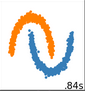
\includegraphics{example_clustering}
    \centering
    \caption{Example of clustering for $d=2$, $m=2$, color represents class.}
\end{figure}

\subsection{Stepwise iterative maximum likelyhood algorithm}
To distinguish different read profiles a new method of clustering was developed.
\subsection{Likelihood}

Assume that the data consists of different multidimensional normal distributions. \\
Let's denote data as  
$$X = \{x_i | x_i \in \mathbb{R}^d, i \in \left( 1 \ldots n \right) \}, m \in \mathbb{N}$$
where $m$ is number of clusters and $n$ number of points. 
Assume that we have some clustering $C$, we will try to increase it's likelihood. \\
Denote ith claster as $\omega_i$ and it's estimated parameters as $\theta_i$
$$ \Theta = \{ \theta_i | i \in (1 \ldots n)\}.$$
Then probability of $x$ in ith cluster
$$ p(x | \Theta) = p(x | \omega_i, \theta_i) P(\omega_i).$$
Denote clusters as $ \chi_1 \ldots \chi_l \subset X $, 
than logarithm of probability for all points in cluster i is 
\begin{align*}
    L_i &= \sum_{x \in \chi_i} \log(p(x| \omega_i, \theta_i)P(\omega_i)) \\
        &=  \log \left( 
        \frac{ \exp \left( \frac{-1}{2} (x - \mu_i)^T \Sigma_i^{-1} (x - \mu_i) \right) }
        {(2 \pi)^{d/2} |\Sigma_i| ^ {1/2}}
        \right) + n_i \log(P(\omega_i)) \\
        &= -\frac{1}{2} n_i d - \frac{n_i d}{2} \log(2 \pi) - \frac{n_i}{2} \log |\Sigma_i| + n_i \log \frac{n_i}{n}.
\end{align*} 
Where $\mu_i$ is mean value and $\Sigma_i$ - covariation of ith cluster.
Overall likelihood is 
$$ L = \sum_{i = 1}^l L_i.$$
Move $\hat{x}$ from $\chi_i$ to $\chi_j$, then

\begin{align*}
    \Delta L_i = &-\frac{1}{2} \log |\Sigma_i| + \frac{n_i - 1}{2} 
        \log \left(1 - \frac{(\hat{x} - \mu_i)^T \Sigma_i^{-1}(\hat{x} - \mu)}{n_i - 1} \right) + \\
         &+ \log \frac{n_i}{n} - (n_i - 1)(\frac{d}{2} + 1) \log \frac{n_i - 1}{n_i}
\end{align*}

\begin{align*}
    \Delta L_j = &-\frac{1}{2} \log |\Sigma_j| - \frac{n_j + 1}{2} 
        \log \left(1 + \frac{(\hat{x} - \mu_j) \Sigma_j^{-1} (\hat{x} - \mu_j)}{n_j + 1}\right) + \\
         &+ \log \frac{n_j}{n} + (n_j + 1)(\frac{d}{2} + 1) \log \frac{n_j + 1}{n_j}.
\end{align*}

\begin{align*}
    \Delta L &= \Delta L_i + \Delta L_j
\end{align*}

\subsection{Algorithm}
Main idea
\begin{enumerate}
    \item Initialize clusters (randomly or using another algorithm)
    \item Iterate over all points
    \begin{enumerate}
        \item Move point to a cluster, such that overall likelihood increases the most. (With most $\Delta L_j$)
        \item Update clusters and their parameters.
    \end{enumerate}
    \item Repeat step 2 while it makes changes.
\end{enumerate}
Advantages
\begin{itemize}
    \item After every step overall likelihood increases.
    \item This implies that the cycle will end.
\end{itemize}
Problems
\begin{itemize}
    \item Updateting parameters after every step is very slow.
\end{itemize}
Transition of one point does not change estimated parameters significantly, 
so to reduce iteration complexity, we will update parameters once in $k$ points. 
Also to avoid possible loops we will iterate over points in different orders. \\
Final algorithm
\begin{enumerate}
    \item Initialize clusters and estimate their parameters
    \item Devide $X$ into $p$ random disjoined groups $g_1 \ldots g_p$.
    \item Loop c from $1$ to $p$.
    \begin{enumerate}
        \item Loop $x$ over $g_c$.
        \item Let $x$ currently be in cluster $i$.
        \begin{enumerate}
            \item If $n_i <= 1$, then pass to next point.
            \item Calculate $\delta_{j}=
                \left\{\begin{array}{cc}
                \Delta L_{j}, & j \neq i \\
                \Delta L_{i}, & j=i
                \end{array}\right. $
            \item Trasfer $x$ to $\argmax (\delta_j)$ cluster.
        \end{enumerate} 
        \item Update parameters.
        \item If overall likelihood decreased, revert changes.
    \end{enumerate}
    \item If any changes were made, repeat step 2.
\end{enumerate}

\section{Main results}
\subsection{Clustering}
\myworries{Examples of clustering reads with likelyhood information}
\subsection{Longshot}
\myworries{Added longshot features}

\newpage
\begin{thebibliography}{00}
    \bibitem{longshot}
    Longshot is variant calling tool for long reads based on pair-Hidden Markov Model.
    \\\texttt{https://www.nature.com/articles/s41467-019-12493-y}
\end{thebibliography}

\end{document}

